\documentclass[12pt, a4paper]{book}

\usepackage{tikz, incgraph, enumitem, amssymb, pifont}

\usetikzlibrary{mindmap, shadows}

\newcommand{\memorizationColor}{red}
\newcommand{\understandingColor}{green}
\newcommand{\steadinessColor}{blue}

\newcommand{\done}{\rlap{$\square$}{\raisebox{2pt}{\large\hspace{1pt}\ding{51}}}\hspace{-2.5pt}}
\newcommand{\wontfix}{\rlap{$\square$}{\raisebox{2pt}{\large\hspace{1pt}\ding{55}}}}

\title{Planner}
\date{November 25, 2022}
\author{Macroactive}

\begin{document}
\begin{inctext}
    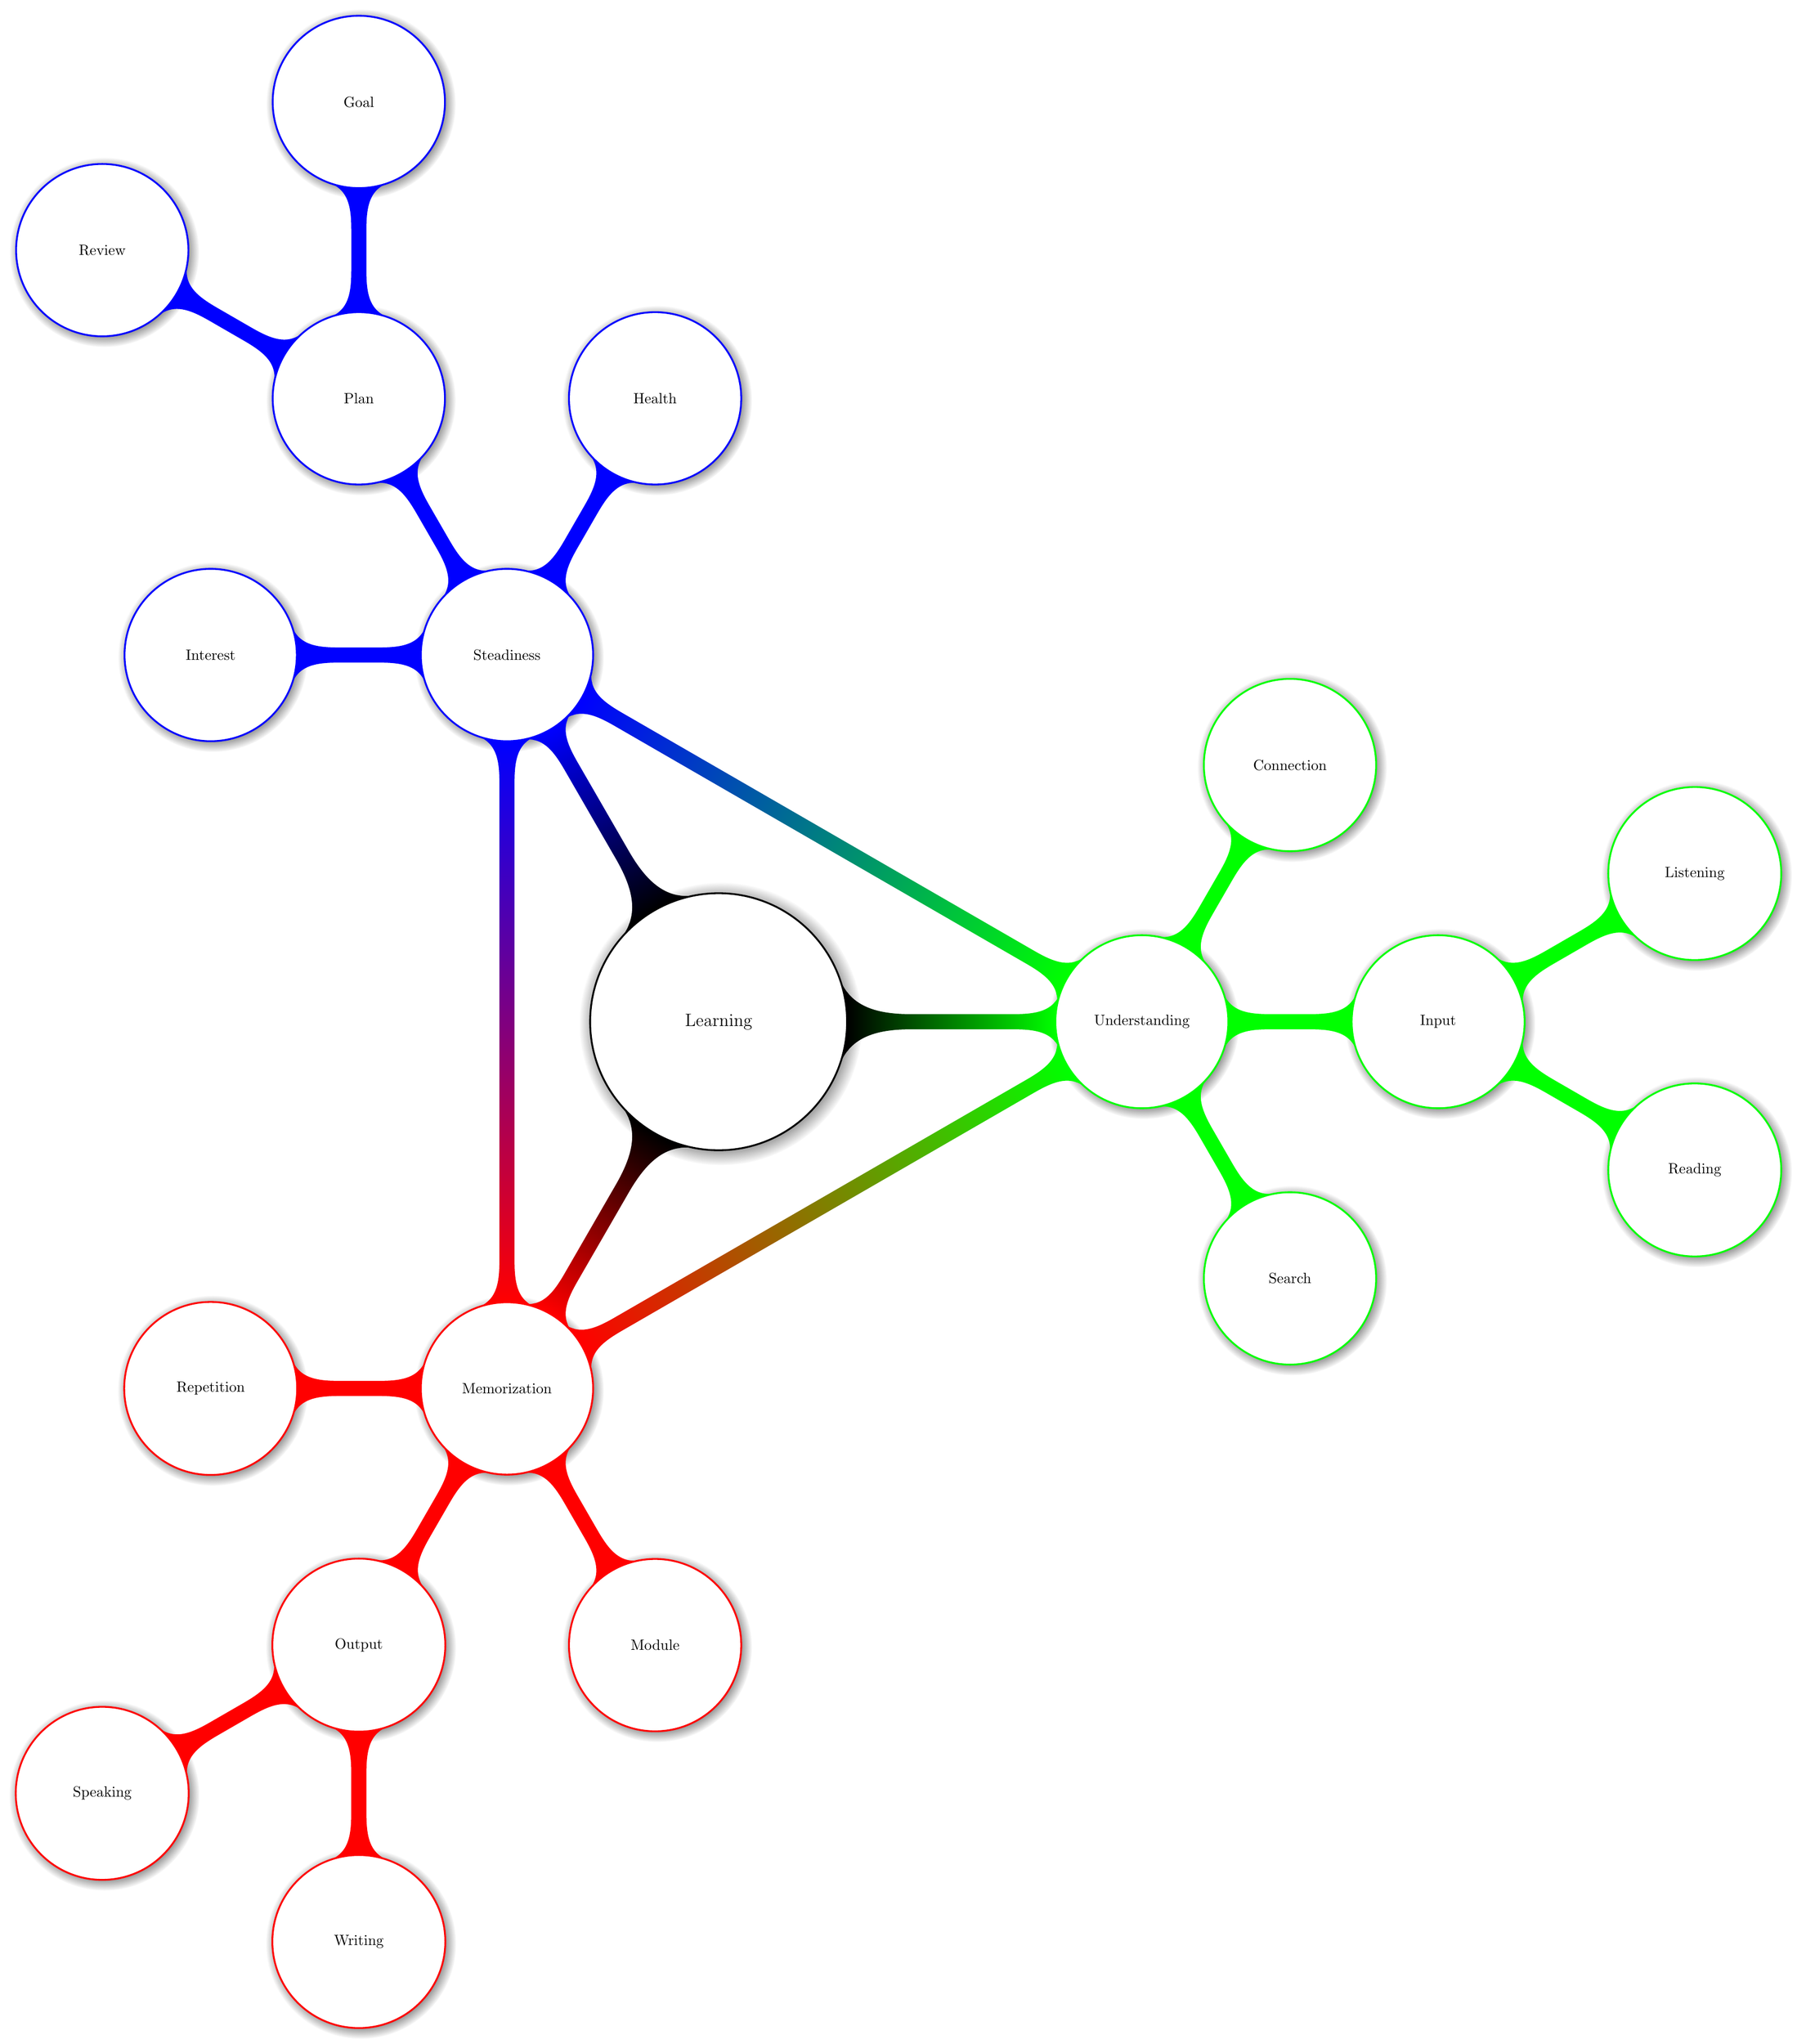
\begin{tikzpicture}[
            mindmap,
            grow cyclic,
            concept color=black,
            every child/.append style={text width=4cm, level distance=7cm, font=\fontsize{10pt}{12pt}},
            every node/.append style={concept, circular drop shadow, fill=white},
            level 1/.append style={sibling angle=120},
            level 3/.append style={sibling angle=60}
        ]
        \node[root concept, text width=6cm]{Learning}
        child[concept color=\memorizationColor, level distance=10cm]{
                node(memorization){
                        Memorization
                    }
                child{
                        node{Repetition}
                    }
                child{
                        node{Output}
                        child{
                                node{Speaking}
                            }
                        child{
                                node{Writing}
                            }
                    }
                child{
                        node{Module}
                    }
            }
        child[concept color=\understandingColor, level distance=10cm]{
                node(understanding){Understanding}
                child{
                        node{Search}
                    }
                child{
                        node{Input}
                        child{
                                node{Reading}
                            }
                        child{
                                node{Listening}
                            }
                    }
                child{
                        node{Connection}
                    }
            }
        child[concept color=\steadinessColor, level distance=10cm]{
                node(steadiness){Steadiness}
                child{
                        node{Health}
                    }
                child{
                        node{Plan}
                        child{
                                node(goal){Goal}
                            }
                        child{
                                node(review){Review}
                            }
                    }
                child{
                        node{Interest}
                    }
            }
        ;
        \path (memorization) to [circle connection bar switch color=from (\memorizationColor!100) to (\understandingColor!100)] (understanding);
        \path (understanding) to [circle connection bar switch color=from (\understandingColor!100) to (\steadinessColor!100)] (steadiness);
        \path (steadiness) to [circle connection bar switch color=from (\steadinessColor!100) to (\memorizationColor!100)] (memorization);

    \end{tikzpicture}
\end{inctext}
{\let\newpage\relax\maketitle}

\newpage
\begin{itemize}
    \item Todo
          \newlist{todoList}{itemize}{2}
          \setlist[todoList]{label=$\square$}
          \begin{todoList}
              \item[\done] Problem 1
              \item Item 3
              \item[\wontfix] Problem 2
          \end{todoList}
\end{itemize}

\end{document}